\documentclass[a4paper]{article}

\usepackage[pdftex,
  hidelinks,
  pdfauthor={Dexter Chua},
  pdfsubject={Cambridge Maths Notes: Part IB - Statistics},
  pdftitle={Part IB - Statistics},
pdfkeywords={Cambridge Mathematics Maths Math IB Lent Statistics}]{hyperref}

% Imports
\ifx \nextra \undefined
  \usepackage[pdftex,
    hidelinks,
    pdfauthor={Dexter Chua},
    pdfsubject={Cambridge Maths Notes: Part \npart\ - \ncourse},
    pdftitle={Part \npart\ - \ncourse},
  pdfkeywords={Cambridge Mathematics Maths Math \npart\ \nterm\ \nyear\ \ncourse}]{hyperref}
  \title{Part \npart\ - \ncourse}
\else
  \usepackage[pdftex,
    hidelinks,
    pdfauthor={Dexter Chua},
    pdfsubject={Cambridge Maths Notes: Part \npart\ - \ncourse\ (\nextra)},
    pdftitle={Part \npart\ - \ncourse\ (\nextra)},
  pdfkeywords={Cambridge Mathematics Maths Math \npart\ \nterm\ \nyear\ \ncourse\ \nextra}]{hyperref}

  \title{Part \npart\ - \ncourse \\ {\Large \nextra}}
\fi

\author{Lectured by \nlecturer \\\small Notes taken by Dexter Chua}
\date{\nterm\ \nyear}

\usepackage{alltt}
\usepackage{amsfonts}
\usepackage{amsmath}
\usepackage{amssymb}
\usepackage{amsthm}
\usepackage{booktabs}
\usepackage{caption}
\usepackage{enumitem}
\usepackage{fancyhdr}
\usepackage{graphicx}
\usepackage{mathtools}
\usepackage{microtype}
\usepackage{multirow}
\usepackage{pdflscape}
\usepackage{pgfplots}
\usepackage{siunitx}
\usepackage{tabularx}
\usepackage{tikz}
\usepackage{tkz-euclide}
\usepackage[normalem]{ulem}
\usepackage[all]{xy}

\pgfplotsset{compat=1.12}

\pagestyle{fancyplain}
\lhead{\emph{\nouppercase{\leftmark}}}
\ifx \nextra \undefined
  \rhead{
    \ifnum\thepage=1
    \else
      \npart\ \ncourse
    \fi}
\else
  \rhead{
    \ifnum\thepage=1
    \else
      \npart\ \ncourse\ (\nextra)
    \fi}
\fi
\usetikzlibrary{arrows}
\usetikzlibrary{decorations.markings}
\usetikzlibrary{decorations.pathmorphing}
\usetikzlibrary{positioning}
\usetikzlibrary{fadings}
\usetikzlibrary{intersections}
\usetikzlibrary{cd}

\newcommand*{\Cdot}{\raisebox{-0.25ex}{\scalebox{1.5}{$\cdot$}}}
\newcommand {\pd}[2][ ]{
  \ifx #1 { }
    \frac{\partial}{\partial #2}
  \else
    \frac{\partial^{#1}}{\partial #2^{#1}}
  \fi
}

% Theorems
\theoremstyle{definition}
\newtheorem*{aim}{Aim}
\newtheorem*{axiom}{Axiom}
\newtheorem*{claim}{Claim}
\newtheorem*{cor}{Corollary}
\newtheorem*{defi}{Definition}
\newtheorem*{eg}{Example}
\newtheorem*{fact}{Fact}
\newtheorem*{law}{Law}
\newtheorem*{lemma}{Lemma}
\newtheorem*{notation}{Notation}
\newtheorem*{prop}{Proposition}
\newtheorem*{thm}{Theorem}

\renewcommand{\labelitemi}{--}
\renewcommand{\labelitemii}{$\circ$}
\renewcommand{\labelenumi}{(\roman{*})}

\let\stdsection\section
\renewcommand\section{\newpage\stdsection}

% Strike through
\def\st{\bgroup \ULdepth=-.55ex \ULset}

% Maths symbols
\newcommand{\bra}{\langle}
\newcommand{\ket}{\rangle}

\newcommand{\N}{\mathbb{N}}
\newcommand{\Z}{\mathbb{Z}}
\newcommand{\Q}{\mathbb{Q}}
\renewcommand{\H}{\mathbb{H}}
\newcommand{\R}{\mathbb{R}}
\newcommand{\C}{\mathbb{C}}
\newcommand{\Prob}{\mathbb{P}}
\renewcommand{\P}{\mathbb{P}}
\newcommand{\E}{\mathbb{E}}
\newcommand{\F}{\mathbb{F}}
\newcommand{\cU}{\mathcal{U}}
\newcommand{\RP}{\mathbb{RP}}
\newcommand{\CP}{\mathbb{CP}}

\newcommand{\ph}{\,\cdot\,}

\DeclareMathOperator{\sech}{sech}
\DeclareMathOperator{\cosech}{cosech}
\DeclareMathOperator{\cosec}{cosec}

\DeclareMathOperator{\covol}{covol}
\DeclareMathOperator{\vol}{vol}

\let\Im\relax
\let\Re\relax
\DeclareMathOperator{\Im}{Im}
\DeclareMathOperator{\Re}{Re}
\DeclareMathOperator{\im}{im}
\DeclareMathOperator{\image}{image}
\DeclareMathOperator{\Ann}{Ann}

\DeclareMathOperator*{\res}{res}
\DeclareMathOperator{\Res}{Res}
\DeclareMathOperator{\Ind}{Ind}

\DeclareMathOperator{\tr}{tr}
\DeclareMathOperator{\diag}{diag}
\DeclareMathOperator{\rank}{rank}
\DeclareMathOperator{\card}{card}
\DeclareMathOperator{\spn}{span}
\DeclareMathOperator{\adj}{adj}

\DeclareMathOperator{\erf}{erf}
\DeclareMathOperator{\erfc}{erfc}

\DeclareMathOperator{\ord}{ord}
\DeclareMathOperator{\Sym}{Sym}

\DeclareMathOperator{\sgn}{sgn}
\DeclareMathOperator{\orb}{orb}
\DeclareMathOperator{\stab}{stab}
\DeclareMathOperator{\ccl}{ccl}

\DeclareMathOperator{\lcm}{lcm}
\DeclareMathOperator{\hcf}{hcf}

\DeclareMathOperator{\Int}{Int}
\DeclareMathOperator{\id}{id}

\DeclareMathOperator{\betaD}{beta}
\DeclareMathOperator{\gammaD}{gamma}
\DeclareMathOperator{\Poisson}{Poisson}
\DeclareMathOperator{\binomial}{binomial}
\DeclareMathOperator{\multinomial}{multinomial}
\DeclareMathOperator{\Bernoulli}{Bernoulli}
\DeclareMathOperator{\like}{like}

\DeclareMathOperator{\var}{var}
\DeclareMathOperator{\cov}{cov}
\DeclareMathOperator{\bias}{bias}
\DeclareMathOperator{\mse}{mse}
\DeclareMathOperator{\corr}{corr}

\DeclareMathOperator{\otp}{otp}
\DeclareMathOperator{\dom}{dom}

\DeclareMathOperator{\Root}{Root}
\DeclareMathOperator{\supp}{supp}
\DeclareMathOperator{\rel}{rel}
\DeclareMathOperator{\Hom}{Hom}
\DeclareMathOperator{\Aut}{Aut}
\DeclareMathOperator{\Gal}{Gal}
\DeclareMathOperator{\Mat}{Mat}
\DeclareMathOperator{\End}{End}
\DeclareMathOperator{\Char}{char}
\DeclareMathOperator{\ev}{ev}
\DeclareMathOperator{\St}{St}
\DeclareMathOperator{\Lk}{Lk}
\DeclareMathOperator{\disc}{disc}
\DeclareMathOperator{\Isom}{Isom}
\DeclareMathOperator{\length}{length}
\DeclareMathOperator{\energy}{energy}
\DeclareMathOperator{\area}{area}
\DeclareMathOperator{\Syl}{Syl}
\DeclareMathOperator{\cl}{cl}
\DeclareMathOperator{\fix}{fix}

\newcommand{\GL}{\mathrm{GL}}
\newcommand{\SL}{\mathrm{SL}}
\newcommand{\PGL}{\mathrm{PGL}}
\newcommand{\PSL}{\mathrm{PSL}}
\newcommand{\PSU}{\mathrm{PSU}}
\newcommand{\Or}{\mathrm{O}}
\newcommand{\SO}{\mathrm{SO}}
\newcommand{\U}{\mathrm{U}}
\newcommand{\SU}{\mathrm{SU}}

\renewcommand{\d}{\mathrm{d}}
\newcommand{\D}{\mathrm{D}}

\tikzset{->/.style = {decoration={markings,
                                  mark=at position 1 with {\arrow[scale=2]{latex'}}},
                      postaction={decorate}}}
\tikzset{<-/.style = {decoration={markings,
                                  mark=at position 0 with {\arrowreversed[scale=2]{latex'}}},
                      postaction={decorate}}}
\tikzset{<->/.style = {decoration={markings,
                                   mark=at position 0 with {\arrowreversed[scale=2]{latex'}},
                                   mark=at position 1 with {\arrow[scale=2]{latex'}}},
                       postaction={decorate}}}
\tikzset{->-/.style = {decoration={markings,
                                   mark=at position #1 with {\arrow[scale=2]{latex'}}},
                       postaction={decorate}}}
\tikzset{-<-/.style = {decoration={markings,
                                   mark=at position #1 with {\arrowreversed[scale=2]{latex'}}},
                       postaction={decorate}}}

\tikzset{circ/.style = {fill, circle, inner sep = 0, minimum size = 3}}
\tikzset{mstate/.style={circle, draw, blue, text=black, minimum width=0.7cm}}

\definecolor{mblue}{rgb}{0.2, 0.3, 0.8}
\definecolor{morange}{rgb}{1, 0.5, 0}
\definecolor{mgreen}{rgb}{0.1, 0.4, 0.2}
\definecolor{mred}{rgb}{0.5, 0, 0}

\def\drawcirculararc(#1,#2)(#3,#4)(#5,#6){%
    \pgfmathsetmacro\cA{(#1*#1+#2*#2-#3*#3-#4*#4)/2}%
    \pgfmathsetmacro\cB{(#1*#1+#2*#2-#5*#5-#6*#6)/2}%
    \pgfmathsetmacro\cy{(\cB*(#1-#3)-\cA*(#1-#5))/%
                        ((#2-#6)*(#1-#3)-(#2-#4)*(#1-#5))}%
    \pgfmathsetmacro\cx{(\cA-\cy*(#2-#4))/(#1-#3)}%
    \pgfmathsetmacro\cr{sqrt((#1-\cx)*(#1-\cx)+(#2-\cy)*(#2-\cy))}%
    \pgfmathsetmacro\cA{atan2(#2-\cy,#1-\cx)}%
    \pgfmathsetmacro\cB{atan2(#6-\cy,#5-\cx)}%
    \pgfmathparse{\cB<\cA}%
    \ifnum\pgfmathresult=1
        \pgfmathsetmacro\cB{\cB+360}%
    \fi
    \draw (#1,#2) arc (\cA:\cB:\cr);%
}
\newcommand\getCoord[3]{\newdimen{#1}\newdimen{#2}\pgfextractx{#1}{\pgfpointanchor{#3}{center}}\pgfextracty{#2}{\pgfpointanchor{#3}{center}}}

\def\Xint#1{\mathchoice
   {\XXint\displaystyle\textstyle{#1}}%
   {\XXint\textstyle\scriptstyle{#1}}%
   {\XXint\scriptstyle\scriptscriptstyle{#1}}%
   {\XXint\scriptscriptstyle\scriptscriptstyle{#1}}%
   \!\int}
\def\XXint#1#2#3{{\setbox0=\hbox{$#1{#2#3}{\int}$}
     \vcenter{\hbox{$#2#3$}}\kern-.5\wd0}}
\def\ddashint{\Xint=}
\def\dashint{\Xint-}


\title{Part IB - Statistics}
\author{Lectured by D. Spiegelhalter}
\date{Lent 2015}

\begin{document}
\maketitle
{\small
\noindent\textbf{Estimation}\\
Review of distribution and density functions, parametric families. Examples: binomial, Poisson, gamma.  Sufficiency, minimal sufficiency, the Rao-Blackwell theorem. Maximum likelihood estimation. Confidence intervals. Use of prior distributions and Bayesian inference.\hspace*{\fill} [5]

\vspace{10pt}
\noindent\textbf{Hypothesis testing}\\
Simple examples of hypothesis testing, null and alternative hypothesis, critical region, size, power, type I and type II errors, Neyman-Pearson lemma. Significance level of outcome. Uniformly most powerful tests. Likelihood ratio, and use of generalised likelihood ratio to construct test statistics for composite hypotheses. Examples, including $t$-tests and $F$-tests. Relationship with confidence intervals. Goodness-of-fit tests and contingency tables.\hspace*{\fill} [4]

\vspace{10pt}
\noindent\textbf{Linear models}\\
Derivation and joint distribution of maximum likelihood estimators, least squares, Gauss-Markov theorem. Testing hypotheses, geometric interpretation. Examples, including simple linear regression and one-way analysis of variance. Use of software.\hspace*{\fill} [7]}

\tableofcontents

\section{Introduction and probability review}
*Lecturer apologizes for not turning up the previous lecture*
\begin{defi}[Statistics]
  \emph{Statistics} is a set of principle a nd procedures for gaining and processing quantitative evidence in order to help us make judgements and decisions.
\end{defi}
Note that we did not mention data. We don't necessarily need data for statistics (even though most often we do).

In this course, we focus on formal \emph{statistical inference}. In the process, we assume
\begin{itemize}
  \item we have data generated from some unknown probability model
  \item we aim to use the data to learn about certain properties of the underlying probability model
\end{itemize}
In particular, we perform parametric inference:

We assume a random variable $X$ takes values in $\mathcal{X}$. We assume its distribution belongs to a family of distribution (e.g. Poisson) indexed by a scalar or vector parameter $\theta$, taking values in some parameter space $\Theta$. We call this a \emph{parametric family}.

For example, we can have $X\sim \text{Poisson}(\mu)$ and $\theta = \mu\in\Theta = (0, \infty)$.

We assume that we already which family it belongs to, and then try to find out $\theta$.

Suppose $X_1, X_2, \cdots, X_n$ are iid with the same distribution as $X$. Then $\mathbf{X} = (X_1, X_2, \cdots, X_n)$ is a simple random sample (i.e. our data).

We use the observed $\mathbf{X} = \mathbf{x}$ to make inferences about $\theta$, such as
\begin{itemize}
  \item giving an estimate $\hat{\theta}(\mathbf{x})$ of the true value of $\theta$.
  \item Giving an interval estimate $(\hat{\theta}_1(\mathbf{x}), \hat{\theta}_2(\mathbf{x}))$ for $\theta$
  \item testing a hypothesis about $\theta$, e.g. whether $\theta = 0$.
\end{itemize}
\section{Estimation, bias and mean squared error}
Suppose that $X_1, \cdots, X_n$ are iid, each with a probability density/mass function $f_X(x|\theta)$. We know $f_X$ but not $\theta$.

\begin{defi}[Statistic]
  A \emph{statistic} is an estimate of $\theta$. It is a function $T$ of a data. If $\mathbf{X} = \mathbf{x} = (x_1, \cdots, x_n)$, then our estimate is written as $\hat{\theta} = T(\mathbf{x})$. $T(\mathbf{X})$ is an \emph{estimator} of $\theta$.

  The distribution of $T = T(\mathbf{X})$ is its sampling distribution.

  Note that capital $\mathbf{X}$ denotes a random variable and $\mathbf{x}$ is an observed value. So $T(\mathbf{X})$ is a random variable and $T(\mathbf{x})$ is a particular value.
\end{defi}

\begin{eg}
  Let $X_1, \cdots, X_n$ is an iid $N(\mu, 1)$. A possible estimator for $\mu$ is
  \[
    T(\mathbf{X}) = \frac{1}{n}\sum X_i.
  \]
  The for any particular observed sample $\mathbf{x}$, our estimate is
  \[
    T(\mathbf{x}) = \frac{1}{n}\sum x_i.
  \]
  Recall that in general, if $X_i \sim N(\mu_i, \sigma_i^2)$, then $\sum X_i \sim N(\sum \mu_i, \sum \sigma_i^2)$, which can be proved by moment-generating functions.
  
  So we have $T(\mathbf{X})\sim N(\mu, 1/n)$. Note that by the Central Limit Theorem, even if $X_1$ were not normal, we still have $T(\mathbf{X})\sim N(\mu, 1/n)$ for large values of $n$.
\end{eg}

\begin{defi}[Bias]
  Let $\hat{\theta} = T(\mathbf{X})$ be an estimator of $\theta$. The \emph{bias} of $\hat{\theta}$ is the difference between its expected value and true value.
  \[
    \bias(\hat{\theta}) = \E_\theta(\hat{\theta}) - \theta.
  \]
  Note that the subscript $_\theta$ does not represent the random variable, but the thing we want to estimate. This is inconsistent with the use for, say the pmf.

  An estimator is \emph{unbiased} if it has no bias, i.e. $\E_\theta(\hat{\theta}) = \theta$.
\end{defi}
To find out $\E_\theta (T)$, we can either find the distribution of $T$ and find its expected value, or evaluate $T$ as a function of $\mathbf{X}$ directly, and find its expected value. 

\begin{eg}
  In the above example, $\E_\mu(T) =\mu$. So $T$ is unbiased for $\mu$. 
\end{eg}
\subsection{Mean squared error}
In general, we prefer estimators whose sampling distributions ``cluster more closely'' around the true value of $\theta$.
\begin{defi}[Mean squared error]
  The \emph{mean squared error} of an estimator $\hat{\theta}$ is $\E_\theta[(\hat{\theta} - \theta)^2]$.

  Sometimes, we use the \emph{root mean squared error}, that is the square root of the above.
\end{defi}
For an unbiased estimator, the mean squared error is just the variance. In general,
\begin{align*}
  \E_\theta[(\hat{\theta} - \theta)^2] &= \E_\theta[(\hat{\theta} - E_\theta(\hat{\theta}) + \E_\theta(\hat{\theta}) - \theta)^2]\\
  &= \E_\theta[(\hat{\theta} - E_\theta(\hat{\theta}))^2] + \E_\theta(\hat{\theta}) - \theta]^2 + 2[\E_\theta(\hat{\theta}) - \theta]\E_\theta[\hat{\theta} - \E_\theta(\hat{\theta})]\\
  &= \var(\hat{\theta}) + \bias^2(\hat{\theta}).
\end{align*}
%complete this
Sometimes it can be preferable to have a biased estimator with a low variance - sometimes know as the ``bias-variance tradeoff''.

For example, suppose $X\sim \binomial(n, \theta)$. The standard estimator is $T_U = \mathbf{X}/n$, which is unbiased. $T_U$ has variance
\[
  \var_\theta(T_U) = \var_\theta(\mathbf{X})/n^2 = \theta(1 - \theta)/n.
\]
Consider an alternative estimator 
\[
  T_B = \frac{X + 1}{n + 2} = w\frac{X}{n} + (1 - w)\frac{1}{2},
\]
where $w = n/(n + 2)$. This can be interpreted to be a weighted average (by the sample size) of the sample mean and $1/2$. We have
\[
  \E_\theta(T_B) - \theta = \frac{n\theta + 1}{n + 2} - \theta = (1 - w)\left(\frac{1}{2} - \theta\right),
\]
and is biased. However,
\[
  \var_\theta(T_B) = \frac{\var_\theta(\mathbf{X})}{(n + 2)^2} = w^2\theta(1 - \theta)/n
\]
Now
\[
  \mse (T_U) = \var_\theta(T_U) + \bias^2(T_U) = \theta(1 - \theta)/n.
\]
and
\[
  \mse (T_B) = \var_\theta(T_B) + \bias^2(T_B) = w^2\frac{\theta(1 - \theta)}{n} + (1 - w)^2\left(\frac{1}{2} - \theta\right)^2
\]
We can plot the mean squared error for possible values of $\theta$. Here we plot the case where $n =1 0$.
\begin{center}
  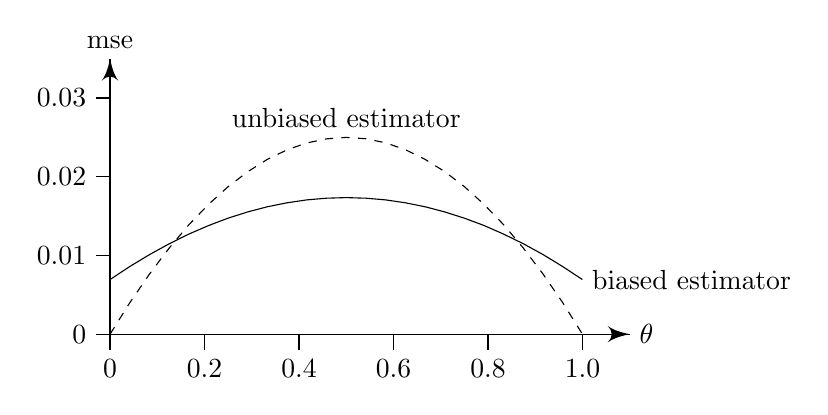
\begin{tikzpicture}[xscale=6,yscale=100]
    \draw [dashed, domain=0:1] plot (\x, {\x * (1 - \x) / 10});
    \node [above] at (0.5, 0.025) {unbiased estimator};
    \draw [domain=0:1] plot (\x, {25 * \x * (1 - \x) / 360 + (1 - 5/6)*(1 - 5/6)*(0.5 - \x)*(0.5 - \x)}) node [right] {biased estimator};
    \draw [->] (0, 0) -- (1.1, 0) node [right] {$\theta$};
    \draw [->] (0, 0) -- (0, 0.035) node [above] {mse};
    \foreach \x in {0, 0.2, 0.4, 0.6, 0.8, 1.0} {
      \draw (\x, 0) -- (\x, -0.002) node [below] {\x};
    }
    \foreach \y in {0, 0.01, 0.02, 0.03} {
      \draw (0, \y) -- (-.03, \y) node [left] {\y};
    }
  \end{tikzpicture}
\end{center}
%plot
We see that this biased estimator has smaller MSE unless $\theta$ has extreme values.

Also, suppose $X\sim \Poisson(\lambda)$, and for some reason, you want to estimate $\theta = [P(\mathbf{X} = 0)]^2 = e^{-2\lambda}$. Then any estimator $T(\mathbf{X})$ must satisfy $\E_\theta(T(\mathbf{X})) = \theta$, or equivalently,
\[
  E_\lambda(T(\mathbf{X})) = e^{-\lambda}\sum_{x = 0}^\infty T(x) \frac{\lambda^x}{x!} = e^{-2\lambda}.
\]
Then the only function $T$ that can satisfy this equation is $T(X) = (-1)^X$.

Then the only unbiased estimator estimate $e^{-2\lambda}$ to be $1$ if $X$ is even, -1 if $X$ is odd. CLEARLY crazy. 
\end{document}
